\documentclass{BeamerTemplate}

\pgfplotsset{compat=1.17}

% Couleurs des barres (deux groupes)
\definecolor{barre1}{HTML}{333333}
\definecolor{barre2}{HTML}{E41A1C}

\pgfplotsset{
  barres/.style={
    ybar, bar width=10pt, ymin=0, enlarge x limits=0.25,
    /pgf/number format/1000 sep={\,},
    tick label style={font=\scriptsize}, label style={font=\small},
    legend style={font=\scriptsize, at={(0.5,1.03)}, anchor=south, draw=none}, legend columns=2,
    legend cell align=left, ymajorgrids, grid style={black!10},
    xtick=data,
  }
}

\title{Chapitre 7 -- Tableaux de fréquences et tests du khi-deux}
\subtitle{STT-1920 Méthodes statistiques}
\date{}

\begin{document}
\begin{frame}[t]
  \titlepage
\end{frame}

\begin{frame}[t]{Plan}
\tableofcontents
\end{frame}

%-------------------------------------------------------------------------------
\section{Test d'adéquation pour une variable discrète}
%-------------------------------------------------------------------------------

\begin{frame}[t]{Test d'adéquation: de quoi s'agit-il?}

\begin{itemize}\itemsep4mm
  \item \textbf{L'objet:} une variable qualitative ou quantitative discrète ayant un
  nombre fini de valeurs possibles.
  \item<2-> \textbf{La question:} le \alert{modèle théorique} de probabilités est-il
  adéquat pour décrire la distribution de cette variable dans la population qui
  nous intéresse?
  \item<3-> \textbf{Le but:} comparer un ensemble d'observations avec les
  \alert{fréquences attendues} sous le modèle théorique pour déterminer si ce
  modèle s'ajuste bien aux données.
\end{itemize}

\end{frame}

\begin{frame}[t]{Exemple 1: les lois de Mendel}

On croise des individus de génotype AAbb avec des individus de génotype aaBB.
Tous les hybrides seront de la forme AaBb.

\begin{itemize}
  \item A et B sont des allèles \alert{dominants} (qui s'expriment avec 1 ou 2 copies);
  \item a et b sont des allèles \alert{récessifs} (qui s'expriment avec 2 copies
  seulement).
\end{itemize}

\medskip
Si on croise des hybrides, il y a 16 génotypes possibles, mais seulement
4 expressions possibles des gènes (\alert{phénotypes}): AB, Ab, aB et ab.

\end{frame}

\begin{frame}[t]{Exemple 1: les lois de Mendel}

Selon les lois de Mendel, qui supposent que les deux gènes ne sont pas liés entre
eux, les quatre phénotypes devraient se retrouver dans la progéniture du
croisement dans les proportions suivantes:

\begin{center}
\renewcommand{\arraystretch}{1.4}
\begin{tabular}{lcccc}
\toprule
Phénotype & AB & Ab & aB & ab\\
\midrule
Proportion théorique & $9/16$ & $3/16$ & $3/16$ & $1/16$\\
\bottomrule
\end{tabular}
\end{center}

\medskip
Que penser de l'hypothèse mendélienne lorsqu'on la confronte aux observations?

\end{frame}

\begin{frame}[t]{Exemple 1: hypothèses}

On veut donc tester les hypothèses suivantes:
\[
H_0: p_1=\tfrac{9}{16},\ p_2=\tfrac{3}{16},\ p_3=\tfrac{3}{16},\ p_4=\tfrac{1}{16}
\qquad
H_1: \text{au moins une des égalités n'est pas vérifiée.}
\]

Il faudra récolter des données dans une population (i.e.\ effectuer plusieurs
croisements et noter le phénotype), et comparer les fréquences observées et
théoriques pour décider si on rejette $H_0$ ou non au seuil $\alpha$.

\uncover<2->{
\begin{Boite}{{Hypothèse nulle, cas général}}
\[
H_0: (p_1,p_2,\ldots,p_J)=(p_1^*,p_2^*,\ldots,p_J^*)
\]
\end{Boite}}

\end{frame}

\begin{frame}[t]{Tableau des fréquences observées}

Le tableau de fréquences donne le nombre de cas observés $(O_1,O_2,\ldots,O_J)$
dans l'échantillon pour chaque valeur de la variable $(v_1,v_2,\ldots,v_J)$.

\bigskip
\begin{center}
\renewcommand{\arraystretch}{1.4}
\begin{tabular}{l|cccc|c}
Valeur & $v_1$ & $v_2$ & $\cdots$ & $v_J$ & Total\\
\hline
Fréquence observée $O_j$ & $O_1$ & $O_2$ & $\cdots$ & $O_J$ & $n$\\
\end{tabular}
\end{center}

\end{frame}

\begin{frame}[t]{Fréquences espérées sous $H_0$}

Les fréquences observées seront comparées aux fréquences attendues sous $H_0$,
donc avec le modèle théorique $(E_1,E_2,\ldots,E_J)$.

\bigskip
\begin{center}
\renewcommand{\arraystretch}{1.4}
\begin{tabular}{l|cccc|c}
Valeur & $v_1$ & $v_2$ & $\cdots$ & $v_J$ & Total\\
\hline
Fréq.\ observée $O_j$ & $O_1$ & $O_2$ & $\cdots$ & $O_J$ & $n$\\
Fréq.\ espérée $E_j$ & $E_1$ & $E_2$ & $\cdots$ & $E_J$ & $n$\\
\end{tabular}
\end{center}

\bigskip
Ces fréquences espérées se calculent comme suit:
\[
E_j = 
\]

\end{frame}

\begin{frame}[t]{Exemple 1: les données}

Voici les résultats d'une expérience effectuée sur 1611 vaches. Quelles sont les
fréquences espérées sous $H_0$, i.e.\ sous l'hypothèse de Mendel?

\bigskip
\begin{center}
\renewcommand{\arraystretch}{1.6}
\begin{tabular}{l|cccc|c}
Phénotype & AB & Ab & aB & ab & Total\\
\hline
Fréq.\ obs.\ ($O_j$) & 926 & 288 & 293 & 104 & 1611\\
Fréq.\ esp.\ ($E_j$) & \hspace{1.2cm} & \hspace{1.2cm} & \hspace{1.2cm}
  & \hspace{1.2cm} & \\
\end{tabular}
\end{center}

\end{frame}

\begin{frame}[t]{Exemple 1: fréquences espérées et observées}

\begin{center}
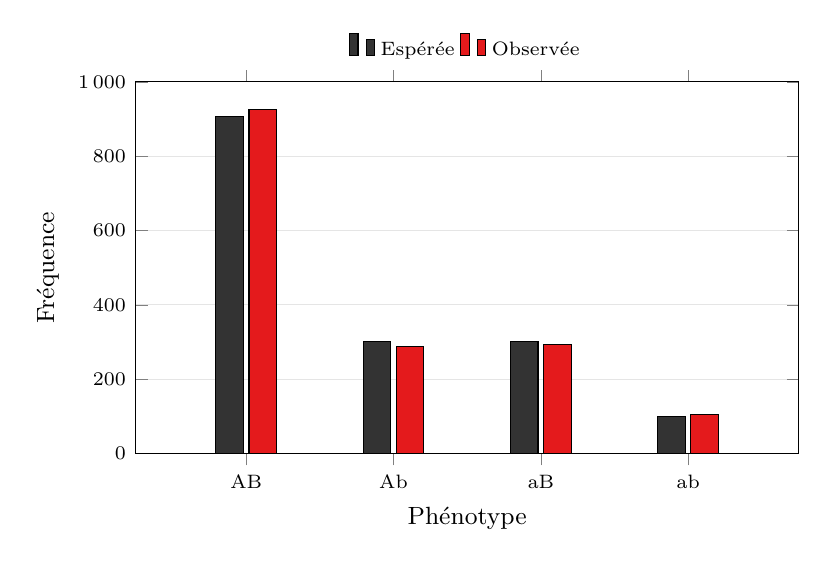
\begin{tikzpicture}
\begin{axis}[barres, width=10cm, height=6.3cm, symbolic x coords={AB,Ab,aB,ab},
  xlabel={Phénotype}, ylabel={Fréquence}, ymax=1000]
  \addplot[fill=barre1, draw=black] coordinates
    {(AB,906.19) (Ab,302.06) (aB,302.06) (ab,100.69)};
  \addplot[fill=barre2, draw=black] coordinates
    {(AB,926) (Ab,288) (aB,293) (ab,104)};
  \legend{Espérée, Observée}
\end{axis}
\end{tikzpicture}
\end{center}

\end{frame}

\begin{frame}[t]{«~Distance~» entre le modèle et les observations}

Pour déterminer à quel point les données et le modèle sont en accord, il faut
comparer les $O_j$ et les $E_j$. Si l'écart est trop grand, on rejettera $H_0$
et on acceptera $H_1$.

\bigskip
\alert{Comment mesure-t-on cet écart?}

\vspace{3cm}

\end{frame}

\begin{frame}[t]{Règle de décision}

\begin{itemize}\itemsep3cm
  \item Si $H_0$ est vraie,
  \item On rejettera donc $H_0$ si\ldots
\end{itemize}

\end{frame}

\begin{frame}[t]{Exemple 1}

Au seuil de 5\,\%, rejette-t-on l'hypothèse de Mendel?

\bigskip
\begin{center}
\renewcommand{\arraystretch}{1.6}
\begin{tabular}{l|cccc|c}
Phénotype & AB & Ab & aB & ab & Total\\
\hline
Fréq.\ obs.\ ($O_j$) & 926 & 288 & 293 & 104 & 1611\\
Fréq.\ esp.\ ($E_j$) & \hspace{1.2cm} & \hspace{1.2cm} & \hspace{1.2cm}
  & \hspace{1.2cm} & \\
Distance & & & & & \\
\end{tabular}
\end{center}

\end{frame}

\begin{frame}[t]{Exemple 1: conclusion}

\vspace{5cm}

\end{frame}

\begin{frame}[t]{Remarques}

\begin{itemize}\itemsep4mm
  \item Ce test est valide si les \alert{fréquences espérées} sont toutes
  supérieures à 5.
  \item Si le modèle théorique est une loi paramétrique (normale, Poisson, etc.)
  dont les paramètres sont estimés à partir des données, la loi du $\chi^2$ perd
  un \alert{degré de liberté supplémentaire} pour chaque paramètre estimé.
\end{itemize}

\end{frame}

%-------------------------------------------------------------------------------
\section{Test d'homogénéité de $I$ populations}
%-------------------------------------------------------------------------------

\begin{frame}[t]{Test d'homogénéité}

On s'intéresse à la distribution d'une variable discrète dans $I$ populations.
On veut savoir si cette distribution est la même pour toutes les populations ou
non, i.e.\ si ces populations sont \alert{homogènes} ou non.

\medskip
\begin{itemize}\itemsep1mm
  \item Distribution de la variable dans la population 1: $(p_{11},p_{12},\ldots,p_{1J})$
  \item Distribution de la variable dans la population 2: $(p_{21},p_{22},\ldots,p_{2J})$
  \item[] $\quad\vdots$
  \item Distribution de la variable dans la population $I$: $(p_{I1},p_{I2},\ldots,p_{IJ})$
\end{itemize}

\end{frame}

\begin{frame}[t]{Les hypothèses du test}

On voudra tester les hypothèses suivantes:
\begin{align*}
H_0&: \text{les } I \text{ distributions sont toutes les mêmes}\\
H_1&: \text{au moins une de ces distributions diffère des autres}
\end{align*}

\begin{itemize}\itemsep1mm
  \item On tire un échantillon de taille $n_1$ dans la population 1;
  \item On tire un échantillon de taille $n_2$ dans la population 2;
  \item[] $\quad\vdots$
  \item On tire un échantillon de taille $n_I$ dans la population $I$.
\end{itemize}

\uncover<2->{Les tailles $n_1,\ldots,n_I$ sont \alert{fixées} par le plan d'échantillonnage.}

\end{frame}

\begin{frame}[t]{Tableau de fréquences}

\begin{center}
\renewcommand{\arraystretch}{1.5}
\begin{tabular}{c|cccc|c}
 & \multicolumn{4}{c|}{Valeurs de la variable} & \\
Population & $v_1$ & $v_2$ & $\cdots$ & $v_J$ & Total\\
\hline
1 & $O_{11}$ & $O_{12}$ & $\cdots$ & $O_{1J}$ & $n_1$\\
2 & $O_{21}$ & $O_{22}$ & $\cdots$ & $O_{2J}$ & $n_2$\\
$\vdots$ & $\vdots$ & $\vdots$ & & $\vdots$ & $\vdots$\\
$I$ & $O_{I1}$ & $O_{I2}$ & $\cdots$ & $O_{IJ}$ & $n_I$\\
\hline
Total & $O_{\bullet1}$ & $O_{\bullet2}$ & $\cdots$ & $O_{\bullet J}$ & $n$\\
\end{tabular}
\end{center}

\end{frame}

\begin{frame}[t]{Exemple 2: vivre seul après le décès du conjoint}

On veut comparer la capacité à vivre seul(e) des hommes et des femmes après le
décès de leur conjoint(e). On obtient des données sur 150 personnes.

\bigskip
\begin{center}
\renewcommand{\arraystretch}{1.3}
\begin{tabular}{l|ccc|c}
 & \multicolumn{3}{c|}{Années vécues après le décès} & \\
Population & $<5$ ans & 5 à 10 ans & $>10$ ans & Total\\
\hline
Hommes (veufs) & 25 & 42 & 33 & 100\\
Femmes (veuves) & 19 & 20 & 11 & 50\\
\hline
Total & 44 & 62 & 44 & 150\\
\end{tabular}
\end{center}

\vfill
{\scriptsize Source: Walpole et Myers, \textit{Probability and Statistics for
Engineers and Scientists}.}

\end{frame}

\begin{frame}[t]{Exemple 2: quel graphique?}

Lequel des deux graphiques ci-dessous illustre le mieux les distributions que
nous souhaitons comparer?

\begin{center}
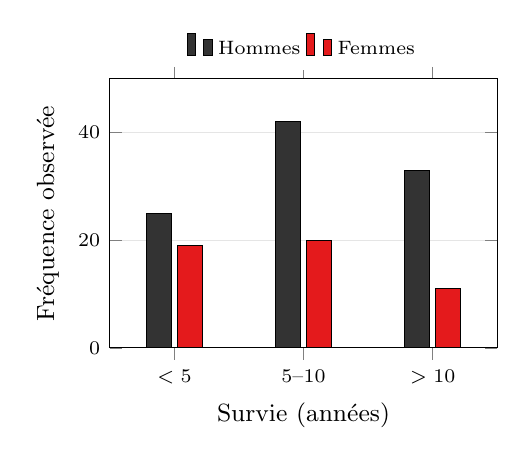
\begin{tikzpicture}
\begin{axis}[barres, width=6.5cm, height=5cm, symbolic x coords={s1,s2,s3},
  xticklabels={$<5$, 5--10, $>10$}, xlabel={Survie (années)},
  ylabel={Fréquence observée}, ymax=50, bar width=9pt]
  \addplot[fill=barre1, draw=black] coordinates {(s1,25) (s2,42) (s3,33)};
  \addplot[fill=barre2, draw=black] coordinates {(s1,19) (s2,20) (s3,11)};
  \legend{Hommes, Femmes}
\end{axis}
\end{tikzpicture}
\hspace{3mm}
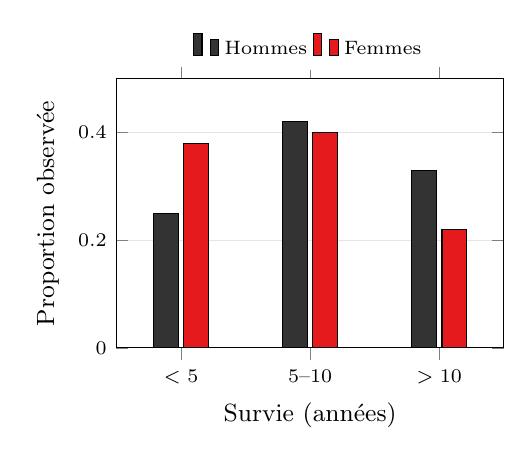
\begin{tikzpicture}
\begin{axis}[barres, width=6.5cm, height=5cm, symbolic x coords={s1,s2,s3},
  xticklabels={$<5$, 5--10, $>10$}, xlabel={Survie (années)},
  ylabel={Proportion observée}, ymax=0.5, bar width=9pt,
  yticklabel style={/pgf/number format/fixed}]
  \addplot[fill=barre1, draw=black] coordinates {(s1,0.25) (s2,0.42) (s3,0.33)};
  \addplot[fill=barre2, draw=black] coordinates {(s1,0.38) (s2,0.40) (s3,0.22)};
  \legend{Hommes, Femmes}
\end{axis}
\end{tikzpicture}
\end{center}

\end{frame}

\begin{frame}[t]{Si $H_0$ était vraie\ldots}

Si $H_0$ est vraie, toutes les distributions théoriques sont homogènes, i.e.\
égales à une distribution commune (inconnue) $p_1,p_2,\ldots,p_J$.

\bigskip
On pourra estimer ces proportions comme suit:
\begin{align*}
\hat p_1 &= \\[2mm]
\hat p_2 &= \\
&\ \,\vdots\\
\hat p_J &=
\end{align*}

\end{frame}

\begin{frame}[t]{Calcul des fréquences espérées}

Si $H_0$ est vraie, on s'attend à ce que:
\begin{align*}
\frac{O_{11}}{n_1}\approx\frac{O_{\bullet1}}{n}
&\quad\Longleftrightarrow\quad O_{11}\approx\\[2mm]
\frac{O_{21}}{n_2}\approx\frac{O_{\bullet1}}{n}
&\quad\Longleftrightarrow\quad O_{21}\approx\\
&\ \ \vdots\\
\frac{O_{ij}}{n_i}\approx\frac{O_{\bullet j}}{n}
&\quad\Longleftrightarrow\quad O_{ij}\approx
\end{align*}

\end{frame}

\begin{frame}[t]{Règle de décision}

Si $H_0$ est vraie,
\[
D=\sum_{i=1}^{I}\sum_{j=1}^{J}\frac{(O_{ij}-E_{ij})^2}{E_{ij}}\ \sim
\]

\vspace{1.5cm}
On rejettera donc $H_0$ si la «~distance~» entre le modèle d'homogénéité et les
observations est trop grande, i.e.\ si\ldots

\end{frame}

\begin{frame}[t]{Exemple 2}

Au seuil de 1\,\%, peut-on dire que la distribution du nombre d'années de vie
est la même chez les hommes et chez les femmes?

\bigskip
\begin{center}
\renewcommand{\arraystretch}{1.3}
\begin{tabular}{l|ccc|c}
 & \multicolumn{3}{c|}{Années vécues après le décès} & \\
Population & $<5$ ans & 5 à 10 ans & $>10$ ans & Total\\
\hline
Hommes (veufs) & 25 & 42 & 33 & 100\\
Femmes (veuves) & 19 & 20 & 11 & 50\\
\hline
Total & 44 & 62 & 44 & 150\\
\end{tabular}
\end{center}

\end{frame}

\begin{frame}[t]{Exemple 2: calcul de la distance}

\[
D=\frac{(O_{11}-E_{11})^2}{E_{11}}+\frac{(O_{12}-E_{12})^2}{E_{12}}+\cdots
\]

\vspace{4cm}

\end{frame}

\begin{frame}[t]{Exemple 2: conclusion}

\vspace{5cm}

\end{frame}

%-------------------------------------------------------------------------------
\section{Test d'indépendance de deux variables discrètes}
%-------------------------------------------------------------------------------

\begin{frame}[t]{Test d'indépendance}

On est ici en présence de \alert{deux variables}, toutes les deux qualitatives ou
quantitatives discrètes, mesurées sur les unités d'un \alert{même échantillon}.
On voudra tester les hypothèses
\begin{align*}
H_0&: \text{les deux variables sont indépendantes}\\
H_1&: \text{les deux variables sont dépendantes.}
\end{align*}

\begin{Boite}{Indépendance}
Deux variables sont indépendantes si le fait de connaître la valeur de l'une des
deux variables ne nous apprend rien sur la valeur de l'autre.
\end{Boite}

\end{frame}

\begin{frame}[t]{Exemple 3: génétique et alcoolisme}

Une étude est menée en Virginie auprès de 1030 paires de femmes jumelles pour
étudier un lien possible entre la génétique et l'alcoolisme. Une entrevue a
permis de classer chaque femme comme ayant une consommation abusive d'alcool ou
non. Voici les résultats.

\medskip
\begin{center}
\renewcommand{\arraystretch}{1.3}
\begin{tabular}{l|*{3}{p{1.4cm}<{\centering}}|c}
 & \multicolumn{3}{c|}{Nb de jumelles avec problème d'alcool} & \\
Jumelles & 0 & 1 & 2 & Total\\
\hline
Identiques & 443 & 102 & 45 & 590\\
Fraternelles & 301 & 113 & 26 & 440\\
\hline
Total & 744 & 215 & 71 & 1030\\
\end{tabular}
\end{center}

\vfill
{\scriptsize K.S.\ Kendler et al., A population-based twin study of alcoholism in
women, \textit{Journal of the American Medical Association}, 268 (1992).}

\end{frame}

\begin{frame}[t]{Exemple 3: sous l'indépendance}

Y a-t-il une relation significative entre le type de jumelles et la présence de
problème d'alcool? Si les variables étaient indépendantes:

\medskip
\begin{itemize}\itemsep3mm
  \item on devrait observer la même proportion de paires sans problème d'alcool
  parmi les jumelles identiques que parmi les jumelles fraternelles
  (i.e.\ $744/1030\approx0{,}72$);
  \item<2-> on devrait observer la même proportion de jumelles identiques parmi
  les paires sans problème d'alcool que parmi celles avec problème d'alcool
  (i.e.\ $590/1030\approx0{,}57$).
\end{itemize}

\end{frame}

\begin{frame}[t]{Exemple 3: quelle est votre impression?}

\begin{center}
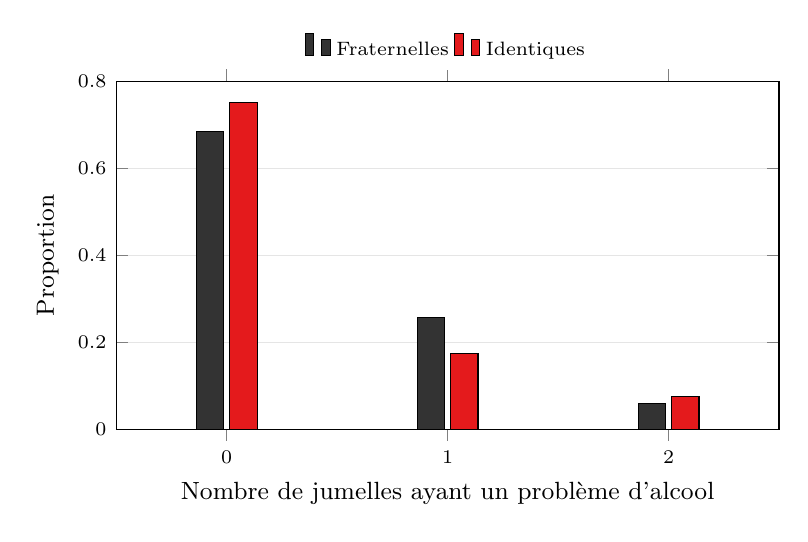
\begin{tikzpicture}
\begin{axis}[barres, width=10cm, height=6cm, symbolic x coords={a0,a1,a2}, xticklabels={0,1,2},
  xlabel={Nombre de jumelles ayant un problème d'alcool}, ylabel={Proportion},
  ymax=0.8, yticklabel style={/pgf/number format/fixed}]
  \addplot[fill=barre1, draw=black] coordinates {(a0,0.684) (a1,0.257) (a2,0.059)};
  \addplot[fill=barre2, draw=black] coordinates {(a0,0.751) (a1,0.173) (a2,0.076)};
  \legend{Fraternelles, Identiques}
\end{axis}
\end{tikzpicture}
\end{center}

\end{frame}

\begin{frame}[t]{Tableau de fréquences}

\begin{center}
\renewcommand{\arraystretch}{1.5}
\begin{tabular}{c|cccc|c}
 & \multicolumn{4}{c|}{Valeurs de la variable 2} & \\
Variable 1 & $v_1$ & $v_2$ & $\cdots$ & $v_J$ & Total\\
\hline
$u_1$ & $O_{11}$ & $O_{12}$ & $\cdots$ & $O_{1J}$ & $O_{1\bullet}$\\
$u_2$ & $O_{21}$ & $O_{22}$ & $\cdots$ & $O_{2J}$ & $O_{2\bullet}$\\
$\vdots$ & $\vdots$ & $\vdots$ & & $\vdots$ & $\vdots$\\
$u_I$ & $O_{I1}$ & $O_{I2}$ & $\cdots$ & $O_{IJ}$ & $O_{I\bullet}$\\
\hline
Total & $O_{\bullet1}$ & $O_{\bullet2}$ & $\cdots$ & $O_{\bullet J}$ & $n$\\
\end{tabular}
\end{center}

\uncover<2->{Ici, seule la taille totale $n$ est fixée à l'avance.}

\end{frame}

\begin{frame}[t]{Calcul des fréquences espérées}

Si $H_0$ est vraie, on s'attend à ce que:
\begin{align*}
\frac{O_{11}}{O_{1\bullet}}\approx\frac{O_{\bullet1}}{n}
&\quad\Longleftrightarrow\quad O_{11}\approx\\[2mm]
\frac{O_{21}}{O_{2\bullet}}\approx\frac{O_{\bullet1}}{n}
&\quad\Longleftrightarrow\quad O_{21}\approx\\
&\ \ \vdots\\
\frac{O_{ij}}{O_{i\bullet}}\approx\frac{O_{\bullet j}}{n}
&\quad\Longleftrightarrow\quad O_{ij}\approx
\end{align*}

\end{frame}

\begin{frame}[t]{Règle de décision}

Si $H_0$ est vraie,
\[
D=\sum_{i=1}^{I}\sum_{j=1}^{J}\frac{(O_{ij}-E_{ij})^2}{E_{ij}}\ \sim
\]

\vspace{1.5cm}
On rejettera donc $H_0$ si la «~distance~» entre le modèle d'indépendance et
les observations est trop grande, i.e.\ si\ldots

\end{frame}

\begin{frame}[t]{Exemple 3}

\small
Peut-on dire au seuil de 5\,\% que la relation entre le type de jumelles et la
présence de problème d'alcool est significative?

\medskip
\begin{center}
\renewcommand{\arraystretch}{1.15}
\begin{tabular}{l|ccc|c}
 & \multicolumn{3}{c|}{Problème d'alcool} & \\
Jumelles & 0 & 1 & 2 & Total\\
\hline
Identiques & 443 & 102 & 45 & 590\\
 & \textcolor{burntorange}{426,2} & \textcolor{burntorange}{123,16} & & \\
 & \textcolor{blue}{0,66} & \textcolor{blue}{3,63} & & \\
\hline
Fraternelles & 301 & 113 & 26 & 440\\
 & \textcolor{burntorange}{317,8} & \textcolor{burntorange}{91,84} & & \\
 & \textcolor{blue}{0,89} & \textcolor{blue}{4,87} & & \\
\hline
Total & 744 & 215 & 71 & 1030\\
\end{tabular}
\end{center}

{\scriptsize Dans chaque case: fréquence observée $O_{ij}$,
\textcolor{burntorange}{fréquence espérée $E_{ij}$} et
\textcolor{blue}{contribution $(O_{ij}-E_{ij})^2/E_{ij}$}.}

\end{frame}

\begin{frame}[t]{Exemple 3: conclusion}

\vspace{5cm}

\end{frame}

\begin{frame}[t]{Question}

Si le but de l'étude est d'étudier l'existence d'un lien entre la
\alert{génétique} et l'alcoolisme, est-ce que le test d'indépendance sur ces
données répondait à la question?

\vspace{4cm}

\end{frame}

\begin{frame}[t]{Exemple 3 revisité}

\begin{center}
\renewcommand{\arraystretch}{1.3}
\begin{tabular}{l|cc|c}
 & \multicolumn{2}{c|}{Jumelles ayant un problème d'alcool} & \\
Jumelles & 0 ou 2 (concordantes) & 1 (discordantes) & Total\\
\hline
Identiques & 488 & 102 & 590\\
Fraternelles & 327 & 113 & 440\\
\hline
Total & 815 & 215 & 1030\\
\end{tabular}
\end{center}

\vspace{3cm}

\end{frame}

\begin{frame}[fragile,t]{En R}

Test d'adéquation (exemple 1):
\begin{Verbatim}[fontsize=\scriptsize]
> chisq.test(c(926, 288, 293, 104), p = c(9, 3, 3, 1)/16)
X-squared = 1.4687, df = 3, p-value = 0.6895
\end{Verbatim}

Test d'homogénéité ou d'indépendance (exemple 3):
\begin{Verbatim}[fontsize=\scriptsize]
> jumelles <- matrix(c(443, 102, 45, 301, 113, 26), nrow = 2, byrow = TRUE)
> test <- chisq.test(jumelles)
> test
X-squared = 11.141, df = 2, p-value = 0.003808
> test$expected     # fréquences espérées
\end{Verbatim}

\small
Dans R Commander: menu \textsf{Statistiques} $\rightarrow$ \textsf{Tableaux de
contingence} $\rightarrow$ \textsf{Saisir et analyser un tableau à double entrée}.

\end{frame}

\begin{frame}[t]{Réponses}

\scriptsize
\begin{itemize}\itemsep1mm
  \item $E_j=np_j^*$. \textbf{Exemple 1:} $E=(906{,}19;\ 302{,}06;\ 302{,}06;\ 100{,}69)$.
  \item Distance: $D=\sum_j (O_j-E_j)^2/E_j$. Si $H_0$ est vraie,
  $D\approx\chi^2_{J-1}$; on rejette $H_0$ si $D>\chi^2_{J-1;\,\alpha}$.
  \item \textbf{Exemple 1:} contributions $0{,}43;\ 0{,}65;\ 0{,}27;\ 0{,}11$, donc
  $D=1{,}47<\chi^2_{3;\,0{,}05}=7{,}81$ (valeur-p $=0{,}69$): on ne rejette pas
  l'hypothèse de Mendel.
  \item \textbf{Exemple 2:} le graphique des \emph{proportions} (les tailles
  d'échantillon diffèrent). $\hat p_j=O_{\bullet j}/n$ et
  $E_{ij}=n_iO_{\bullet j}/n$. Sous $H_0$, $D\approx\chi^2_{(I-1)(J-1)}$.
  $E$: hommes $29{,}33;\ 41{,}33;\ 29{,}33$; femmes $14{,}67;\ 20{,}67;\ 14{,}67$.
  $D=3{,}33<\chi^2_{2;\,0{,}01}=9{,}21$ (valeur-p $=0{,}19$): on ne rejette pas
  l'homogénéité.
  \item \textbf{Exemple 3:} $E_{ij}=O_{i\bullet}O_{\bullet j}/n$; $E_{13}=40{,}67$,
  $E_{23}=30{,}33$ (contributions $0{,}46$ et $0{,}62$). $D=11{,}14>\chi^2_{2;\,0{,}05}=5{,}99$
  (valeur-p $=0{,}004$): relation significative.
  \item \textbf{Question:} pas directement; le lien génétique se manifeste par la
  \emph{concordance} des jumelles (0 ou 2) plus fréquente chez les identiques.
  \item \textbf{Revisité:} $D=10{,}75>\chi^2_{1;\,0{,}05}=3{,}84$ (valeur-p $=0{,}001$):
  les jumelles identiques sont plus souvent concordantes.
\end{itemize}

\end{frame}

\end{document}
